\begin{figure}[htbp]
    \centering
    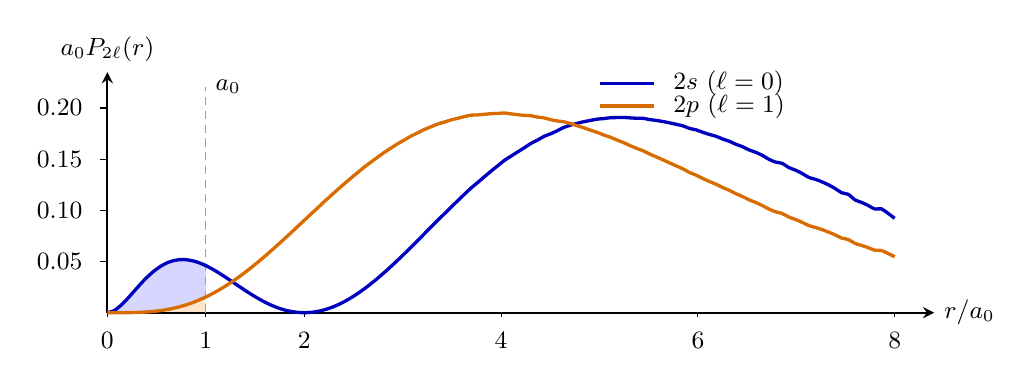
\begin{tikzpicture}[>=stealth, every node/.style={font=\small},x=1.25cm,y=13cm]
        \fill[blue!16]
            plot[domain=0:1,samples=30] (\x,{\x*\x*(2-\x)*(2-\x)*exp(-\x)/8})
            -- (1,0) -- (0,0) -- cycle;
        \fill[orange!20]
            plot[domain=0:1,samples=30] (\x,{\x*\x*\x*\x*exp(-\x)/24})
            -- (1,0) -- (0,0) -- cycle;
        \draw[->,thick] (0,0) -- (8.4,0) node[right] {$r/a_0$};
        \draw[->,thick] (0,0) -- (0,0.235) node[above] {$a_0P_{2\ell}(r)$};
        \foreach \x in {0,1,2,4,6,8}
            \draw (\x,0) -- (\x,-0.004) node[below=2pt] {\x};
        \foreach \y/\lab in {0.05/0.05,0.10/0.10,0.15/0.15,0.20/0.20}
            \draw (0,\y) -- (-0.07,\y) node[left=3pt] {\lab};
        \draw[densely dashed,gray!75] (1,0) -- (1,0.22);
        \node[above right] at (1,0.205) {$a_0$};
        \draw[very thick,blue!75!black,domain=0:8,samples=120,smooth]
            plot (\x,{\x*\x*(2-\x)*(2-\x)*exp(-\x)/8});
        \draw[very thick,orange!85!black,domain=0:8,samples=120,smooth]
            plot (\x,{\x*\x*\x*\x*exp(-\x)/24});
        \draw[blue!75!black,very thick] (5.0,0.224) -- (5.55,0.224);
        \node[anchor=west] at (5.65,0.224) {$2s\ (\ell=0)$};
        \draw[orange!85!black,very thick] (5.0,0.202) -- (5.55,0.202);
        \node[anchor=west] at (5.65,0.202) {$2p\ (\ell=1)$};
    \end{tikzpicture}
    \caption{Densidades radiales $P_{2\ell}(r)=r^2|R_{2\ell}(r)|^2$ en unidades adimensionales. El área sombreada entre el origen y $a_0$ representa las probabilidades $P_{2s}\simeq0.0343$ y $P_{2p}\simeq0.00366$; el estado $2s$ es unas $9.38$ veces más probable en esa región.}
    \label{fig:probabilidad-radial}
\end{figure}